\documentclass[t,dvipsnames,table]{beamer}
\usetheme{Copenhagen}
\setbeamertemplate{headline}{} % remove toc from headers
\beamertemplatenavigationsymbolsempty

\usepackage{amsmath, array, tikz, xcolor, tcolorbox, bm, tkz-euclide, pgfplots, graphicx}
\pgfplotsset{compat = 1.16}
\usetkzobj{all}
\everymath{\displaystyle}

\title{Ellipses}
\author{}
\date{}

\AtBeginSection[]
{
  \begin{frame}
    \frametitle{Objectives}
    \tableofcontents[currentsection]
  \end{frame}
}

\begin{document}

\begin{frame} 
\maketitle
\end{frame}

\begin{frame}[c]
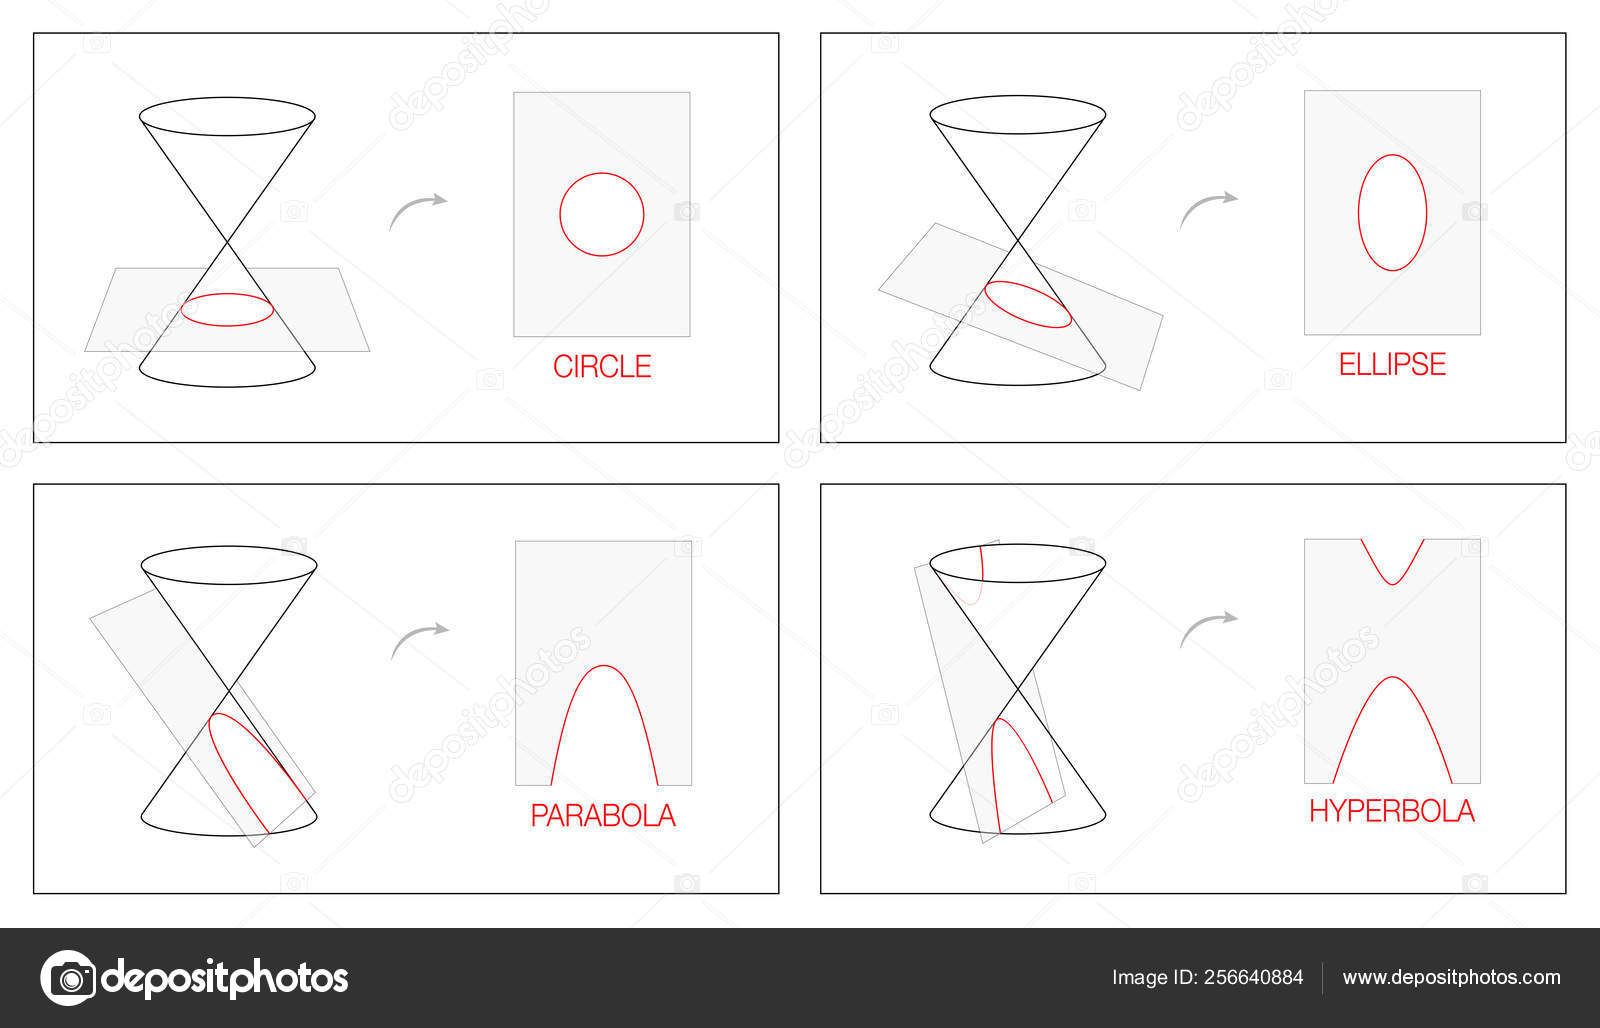
\includegraphics[scale=0.80]{Images/conics.jpg}
\end{frame}

\section{Identify the center, vertices, and foci of an ellipse.}

\begin{frame}{Ellipses}
\begin{tcolorbox}[colback=red!10!white, colframe=red!60!black,, title=\textbf{Ellipses}]
The set of points such that the \textbf{sum} of their distances from 2 fixed points (called \textbf{foci}) is constant.
\end{tcolorbox}
\end{frame}

\begin{frame}{Appearance}
Ellipses will typically either appear wider or taller based on their equation. Below are key parts of each type of ellipse:
	\begin{center}
    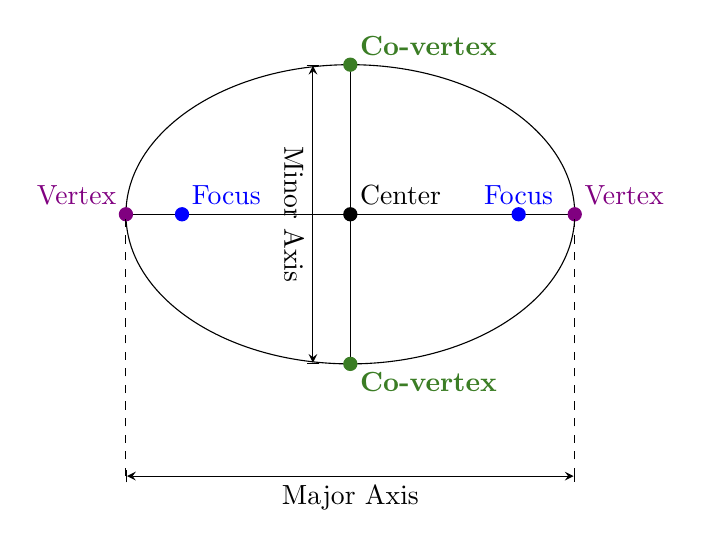
\begin{tikzpicture}[scale=0.95]
    \draw [] (-3,0) -- (3,0);
    \draw [] (0,-2) -- (0,2);
    \draw (0,0) ellipse (3cm and 2cm);
    \draw [fill=black] (0,0) circle (2.5pt);
    \node at (0,0) [anchor=south west] {Center};
    \draw [color=violet, fill=violet] (3,0) circle (2.5pt);
    \node at (3,0) [anchor=south west, color=violet] {Vertex};
    \draw [color=violet, fill=violet] (-3,0) circle (2.5pt);
    \node at (-3,0) [anchor=south east, color=violet] {Vertex};
    \draw [fill=blue, color=blue] (-2.25,0) circle (2.5pt);
    \node at (-2.25,0) [anchor=south west] {\color{blue}Focus};
    \draw [fill=blue, color=blue] (2.25,0) circle (2.5pt);
    \node at (2.25,0) [anchor=south] {\color{blue}Focus};
    \draw [color=OliveGreen, fill=OliveGreen] (0,2) circle (2.5pt);
    \node at (0,2.25) [anchor=south west, color=OliveGreen, yshift=-0.25cm] {\textbf{Co-vertex}};
    \draw [color=OliveGreen, fill=OliveGreen] (0,-2) circle (2.5pt);
    \node at (0,-2.25) [anchor=north west, color=OliveGreen, yshift=0.25cm] {\textbf{Co-vertex}};
    \draw [|<->|, >=stealth] (-3,-3.5) -- (3,-3.5);
    \draw [dashed] (-3,-3.5) -- (-3,0); 
    \draw [dashed] (3,-3.5) -- (3,0);
    \node at (0,-3.5) [anchor=north] {Major Axis};
    \draw [|<->|, >=stealth] (-0.5,-2) -- (-0.5,2);
    \node at (-0.5,0) [rotate=270, anchor=north] {Minor Axis};
\end{tikzpicture}
\end{center}
\end{frame}

\begin{frame}{Appearance}
\begin{center}
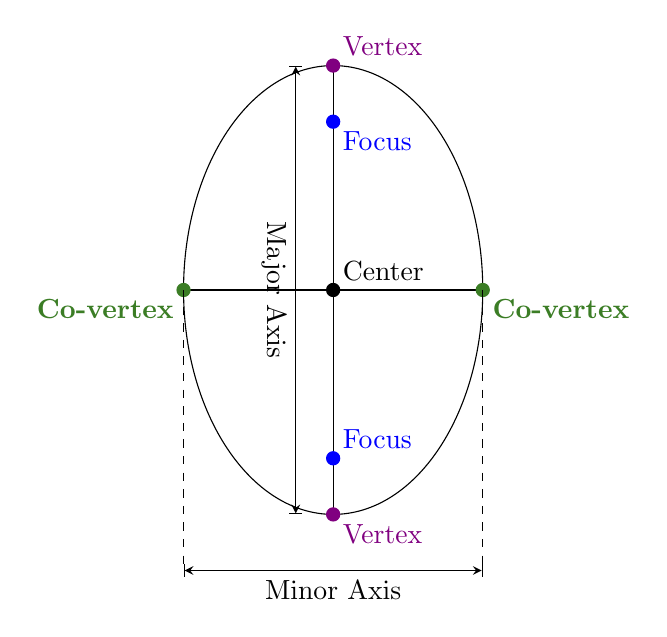
\begin{tikzpicture}[scale=0.95]
    \draw (-2,0) -- (2,0);
    \draw (0,-3) -- (0,3);
    \draw (0,0) ellipse (2cm and 3cm);
    \draw [fill=black] (0,0) circle (2.5pt);
    \node at (0,0) [anchor=south west] {Center};
    \draw [color=violet, fill=violet] (0,3) circle (2.5pt);
    \node at (0,3) [anchor=south west, color=violet] {Vertex};
    \draw [color=violet, fill=violet] (0,-3) circle (2.5pt);
    \node at (0,-3) [anchor=north west, color=violet] {Vertex};
    \draw [fill=blue, color=blue] (0,-2.25) circle (2.5pt);
    \node at (0,-2.25) [anchor=south west] {\color{blue}Focus};
    \draw [fill=blue, color=blue] (0,2.25) circle (2.5pt);
    \node at (0,2.25) [anchor=north west] {\color{blue}Focus};
    \draw [color=OliveGreen, fill=OliveGreen] (2,0) circle (2.5pt);
    \node at (2,0) [anchor=north west, color=OliveGreen] {\textbf{Co-vertex}};
    \draw [color=OliveGreen, fill=OliveGreen] (-2,0) circle (2.5pt);
    \node at (-2,0) [anchor=north east, color=OliveGreen] {\textbf{Co-vertex}};
    \draw [|<->|, >=stealth] (-0.5,3) -- (-0.5,-3);
    \node at (-0.5,0) [rotate=270, anchor=north] {Major Axis};
    \draw [|<->|, >=stealth] (-2,-3.75) -- (2,-3.75);
    \node at (0,-3.75) [anchor=north] {Minor Axis};
    \draw [dashed] (-2,0) -- (-2,-3.75);
    \draw [dashed] (2,0) -- (2,-3.75);
\end{tikzpicture}
\end{center}
\end{frame}

\begin{frame}{Vocab}
The \emph{center} of an ellipse is denoted by $(h, k)$, just like with circles.    \newline\\	\pause 

Each focal point (\textit{pl: foci}) is $c$ units from the center. The foci are on the \emph{major axis}.  \newline\\ \pause 

Each vertex (\textit{pl: vertices}) also lies on the major axis, and is $a$ units away from the center. \newline\\ \pause 

Each \emph{co-vertex} (\textit{pl: co-vertices}) lies on the \emph{minor axis}, which is perpendicular to the major axis. The co-vertices are each $b$ units away from the center.
\end{frame}

\begin{frame}{$\dfrac{(x-h)^2}{a^2} + \dfrac{(y-k)^2}{b^2} = 1$}
\begin{center}
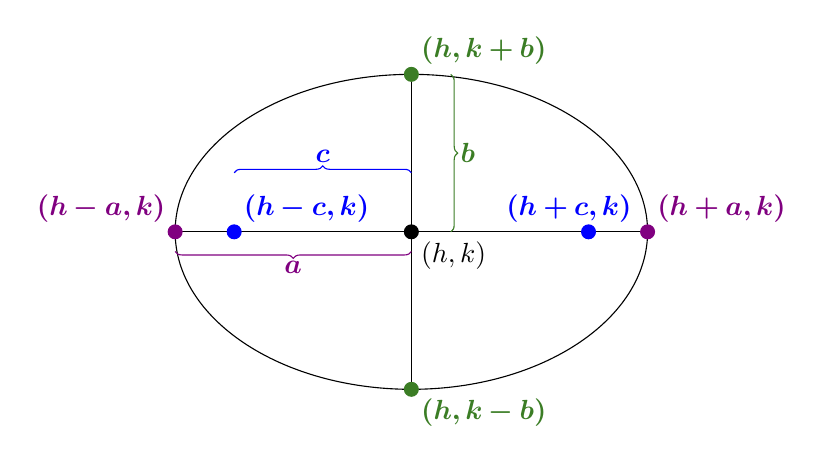
\begin{tikzpicture}
    \draw [] (-3,0) -- (3,0);
    \draw [] (0,-2) -- (0,2);
    \draw (0,0) ellipse (3cm and 2cm);
    \draw [fill=black] (0,0) circle (2.5pt);
    \node at (0,0) [anchor=north west] {$(h,k)$};
    \draw [color=violet, fill=violet] (3,0) circle (2.5pt);
    \node at (3,0) [anchor=south west, color=violet] {$\bm{(h+a,k)}$};
    \draw [color=violet, fill=violet] (-3,0) circle (2.5pt);
    \node at (-3,0) [anchor=south east, color=violet] {$\bm{(h-a,k)}$};
    \draw [fill=blue, color=blue] (-2.25,0) circle (2.5pt);
    \node at (-2.25,0) [anchor=south west] {\color{blue}$\bm{(h-c,k)}$};
    \draw [fill=blue, color=blue] (2.25,0) circle (2.5pt);
    \node at (2.25,0) [anchor=south, xshift=-0.25cm] {\color{blue}$\bm{(h+c,k)}$};
    \draw [color=OliveGreen, fill=OliveGreen] (0,2) circle (2.5pt);
    \node at (0,2.25) [anchor=south west, color=OliveGreen, yshift=-0.25cm] {$\bm{(h,k+b)}$};
    \draw [color=OliveGreen, fill=OliveGreen] (0,-2) circle (2.5pt);
    \node at (0,-2.25) [anchor=north west, color=OliveGreen, yshift=0.25cm] {$\bm{(h, k-b)}$};
    \draw [decoration={brace}, decorate, color=violet, yshift=-0.25cm] (0,0) -- (-3,0);
    \node at (-1.5,-0.25) [anchor=north, color=violet] {$\bm{a}$};
    \draw [decoration={brace}, decorate, color=OliveGreen, xshift=0.5cm] (0,2) -- (0,0);
    \node at (0.5,1) [anchor=west, color=OliveGreen] {$\bm{b}$};
    \draw [decoration={brace}, decorate, color=blue, yshift=0.75cm] (-2.25,0) -- (0,0);
    \node at (-1.125,0.75) [anchor=south, color=blue] {$\bm{c}$};
\end{tikzpicture}
\end{center}
\end{frame}

\begin{frame}{$\dfrac{(y-k)^2}{a^2} + \dfrac{(x-h)^2}{b^2} = 1$}
\begin{center}
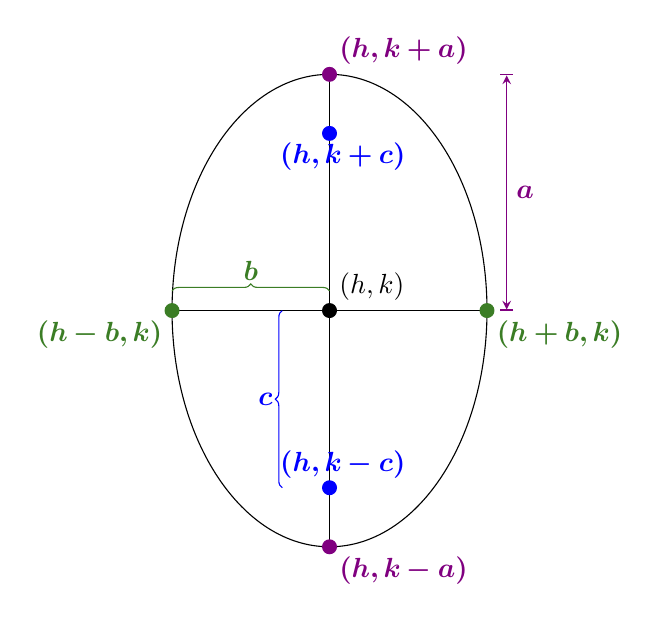
\begin{tikzpicture}
    \draw (-2,0) -- (2,0);
    \draw (0,-3) -- (0,3);
    \draw (0,0) ellipse (2cm and 3cm);
    \draw [fill=black] (0,0) circle (2.5pt);
    \node at (0,0) [anchor=south west] {$(h, k)$};
    \draw [color=violet, fill=violet] (0,3) circle (2.5pt);
    \node at (0,3) [anchor=south west, color=violet] {$\bm{(h, k+a)}$};
    \draw [color=violet, fill=violet] (0,-3) circle (2.5pt);
    \node at (0,-3) [anchor=north west, color=violet] {$\bm{(h, k-a)}$};
    \draw [fill=blue, color=blue] (0,-2.25) circle (2.5pt);
    \node at (0,-2.25) [anchor=south west, xshift=-0.75cm] {\color{blue}$\bm{(h, k-c)}$};
    \draw [fill=blue, color=blue] (0,2.25) circle (2.5pt);
    \node at (0,2.25) [anchor=north west, xshift=-0.75cm] {\color{blue}$\bm{(h, k+c)}$};
    \draw [color=OliveGreen, fill=OliveGreen] (2,0) circle (2.5pt);
    \node at (2,0) [anchor=north west, color=OliveGreen] {$\bm{(h+b,k)}$};
    \draw [color=OliveGreen, fill=OliveGreen] (-2,0) circle (2.5pt);
    \node at (-2,0) [anchor=north east, color=OliveGreen] {$\bm{(h-b,k)}$};
    \draw [decoration={brace}, decorate, yshift=0.25cm, color=OliveGreen] (-2,0) -- (0,0);
    \node at (-1,0.5) [color=OliveGreen] {$\bm{b}$};
    \draw [decoration={brace}, decorate, color=blue, xshift=-0.6cm] (0,-2.25) -- (0,0);
    \node at (-0.6, -1.125) [anchor=east, color=blue] {$\bm{c}$};
    \draw [|<->|, >=stealth, color=violet] (2.25,0) -- (2.25,3);
    \node at (2.25, 1.5) [anchor=west, color=violet] {$\bm{a}$};
\end{tikzpicture}
\end{center}
\end{frame}

\begin{frame}{Foci and $a$ vs. $b$}
\emph{Note:} In both cases, $c^2 = a^2 - b^2$, and $a > b$. 
\end{frame}

\begin{frame}{Example 1}
Identify the coordinates of the center, vertices, and foci for each. Exact answers only.	\newline\\
(a)	\quad $\frac{x^2}{36} + \frac{y^2}{25} = 1$	\newline\\
\onslide<2->{Center: $(0,0)$}	\newline\\
\onslide<3->{Vertices: $a = 36$} 
\onslide<4->{$\longrightarrow a = \pm 6$}	\newline\\
\onslide<5->{Vertices at $(0 \pm 6, 0)$ }	\newline\\
\onslide<6->{Vertices $(\pm 6, 0)$}
\end{frame}

\begin{frame}{Example 1a	\quad $\tfrac{x^2}{36} + \tfrac{y^2}{25} = 1$}
Foci:
\begin{align*}
c^2 &= a^2 - b^2	\\[8pt]
\onslide<2->{c^2 &= 36-25} \\[8pt]
\onslide<3->{c^2 &= 11}	\\[8pt]
\onslide<4->{c &= \pm \sqrt{11}} 
\end{align*}
\onslide<5->{Foci at $(0 \pm \sqrt{11},0)$}
\onslide<6->{$\longrightarrow (\pm \sqrt{11}, 0)$}
\end{frame}


\begin{frame}{Example 1}
(b)	\quad $\frac{y^2}{16} + \frac{x^2}{1} = 1$	\newline\\
\onslide<2->{Center: $(0,0)$}	\newline\\
\onslide<3->{Vertices: $a = 16$} 
\onslide<4->{$\longrightarrow a = \pm 4$}	\newline\\
\onslide<5->{Vertices at $(0, 0 \pm 4)$ }	\newline\\
\onslide<6->{Vertices $(0, \pm 4)$}
\end{frame}

\begin{frame}{Example 1b	\quad $\tfrac{y^2}{16} + \tfrac{x^2}{1} = 1$}
Foci:
\begin{align*}
c^2 &= a^2 - b^2	\\[8pt]
\onslide<2->{c^2 &= 16-1} \\[8pt]
\onslide<3->{c^2 &= 15}	\\[8pt]
\onslide<4->{c &= \pm \sqrt{15}} 
\end{align*}
\onslide<5->{Foci at $(0,0 \pm \sqrt{15})$}
\onslide<6->{$\longrightarrow (0, \pm \sqrt{15})$}
\end{frame}

\begin{frame}{Example 1}
(c)	\quad $\frac{(x+5)^2}{49} + \frac{(y-2)^2}{25} = 1$	\newline\\
\onslide<2->{Center: $(-5,2)$}	\newline\\
\onslide<3->{Vertices: $a = 49$} 
\onslide<4->{$\longrightarrow a = \pm 7$}	\newline\\
\onslide<5->{Vertices at $(-5\pm 7, 2)$ }	\newline\\
\onslide<6->{Vertices $(-12,2) \text{ and } (2,2)$}
\end{frame}

\begin{frame}{Example 1c	\quad $\tfrac{(x+5)^2}{49} + \tfrac{(y-2)^2}{25} = 1$}
Foci:
\begin{align*}
c^2 &= a^2 - b^2	\\[8pt]
\onslide<2->{c^2 &= 49-25} \\[8pt]
\onslide<3->{c^2 &= 24}	\\[8pt]
\onslide<4->{c &= \pm 2\sqrt{6}} 
\end{align*}
\onslide<5->{Foci at $(-5\pm 2\sqrt{6}, 2)$}
\end{frame}

\begin{frame}{Example 1}
(d)	\quad $(x-2)^2 + \frac{(y+1)^2}{36} = 1$	\newline\\
\onslide<2->{Center: $(2,-1)$}	\newline\\
\onslide<3->{Vertices: $a = 36$} 
\onslide<4->{$\longrightarrow a = \pm 6$}	\newline\\
\onslide<5->{Vertices at $(2,-1\pm 6)$ }	\newline\\
\onslide<6->{Vertices $(2,-7) \text{ and } (2,5)$}
\end{frame}

\begin{frame}{Example 1d	\quad $\tfrac{(x-2)^2}{1} + \tfrac{(y+1)^2}{36} = 1$}
Foci:
\begin{align*}
c^2 &= a^2 - b^2	\\[8pt]
\onslide<2->{c^2 &= 36-1} \\[8pt]
\onslide<3->{c^2 &= 35}	\\[8pt]
\onslide<4->{c &= \pm \sqrt{35}} 
\end{align*}
\onslide<5->{Foci at $(2, -1\pm \sqrt{35})$}
\end{frame}


\section{Write the equation of an ellipse in standard form.}

\begin{frame}{Converting From General to Standard Form}
Just like circles may not be written in standard form, you may need to find the center and vertices to write an ellipse in standard form. \newline\\ \pause 

Luckily, the process is similar to that for circles.
\end{frame}

\begin{frame}{Example 2}
Write the standard form for the equation of an ellipse for each of the following.	\newline\\
(a)	\quad	$9x^2 + 16y^2 - 144 = 0$
\begin{align*}
\onslide<2->{9x^2 + 16y^2 - 144 &= 0}	\\[8pt]
\onslide<3->{9x^2 + 16y^2 &= 144} \\[8pt]
\onslide<4->{\frac{9x^2}{144} + \frac{16y^2}{144} &= 1} \\[10pt]
\onslide<5->{\frac{x^2}{16} + \frac{y^2}{9} &= 1}
\end{align*} 
\end{frame}

\begin{frame}{Example 2}
(b)	\quad	$25x^2 + y^2 - 25 = 0 $
\begin{align*}
\onslide<2->{25x^2 + y^2 - 25 &= 0 }	\\[8pt]
\onslide<3->{25x^2 + y^2 &= 25 } \\[8pt]
\onslide<4->{\frac{25x^2}{25} + \frac{y^2}{25} &= 1} \\[10pt]
\onslide<5->{x^2 + \frac{y^2}{25} &= 1}
\end{align*} 
\end{frame}

\begin{frame}{Example 2}
(c)	\quad	$9x^2-54x+4y^2-8y+49 = 0$
\onslide<2->{\[{\color{blue}\bm{9x^2 - 54x}} + {\color{red}\bm{4y^2 - 8y}} = -49\]} 
\onslide<3->{{\color{blue}\textbf{Vertex: }$\bm{(3,-81)}$}}	\newline\\
\onslide<4->{{\color{red}\textbf{Vertex: }$\bm{(1,-4)}$}}
\begin{align*}
\onslide<5->{9(x-3)^2 + 4(y-1)^2 &= -49 + |-81| + |-4|}	\\[8pt]
\onslide<6->{9(x-3)^2 + 4(y-1)^2 &= 36} \\[10pt]
\onslide<7->{\frac{9(x-3)^2}{36} + \frac{4(y-1)^2}{36} &= 1}
\end{align*}
\end{frame}

\begin{frame}{Example 2c}
\begin{align*}
\frac{9(x-3)^2}{36} + \frac{4(y-1)^2}{36} &= 1	\\[18pt]
\onslide<2->{\frac{(x-3)^2}{4} + \frac{(y-1)^2}{9} &= 1}
\end{align*}
\end{frame}


\begin{frame}{Example 2}
(d)	\quad	$x^2+6x+9y^2+18y+9=0$
\onslide<2->{\[{\color{blue}\bm{x^2 + 6x}} + {\color{red}\bm{9y^2 + 18y}} = -9\]} 
\onslide<3->{{\color{blue}\textbf{Vertex: }$\bm{(-3,-9)}$}}	\newline\\
\onslide<4->{{\color{red}\textbf{Vertex: }$\bm{(-1,-9)}$}}
\begin{align*}
\onslide<5->{(x+3)^2 + 9(y+1)^2 &= -9 + |-9| + |-9|}	\\[8pt]
\onslide<6->{(x+3)^2 + 9(y+1)^2 &= 9} \\[10pt]
\onslide<7->{\frac{(x+3)^2}{9} + \frac{9(y-1)^2}{9} &= 1}
\end{align*}
\end{frame}

\begin{frame}{Example 2d}
\begin{align*}
\frac{(x+3)^2}{9} + \frac{9(y-1)^2}{9} &= 1	\\[18pt]
\onslide<2->{\frac{(x+3)^2}{9} + (y-1)^2 &= 1}
\end{align*}
\end{frame}

\end{document}